\documentclass[a4paper,10pt]{article}

% For code example
\usepackage{listings}
\usepackage{xcolor}
\definecolor{codegreen}{rgb}{0,0.6,0}
\definecolor{codegray}{rgb}{0.5,0.5,0.5}
\definecolor{codepurple}{rgb}{0.58,0,0.82}
\definecolor{backcolour}{rgb}{0.95,0.95,0.92}
\lstdefinestyle{mystyle}{
    backgroundcolor=\color{backcolour},   
    commentstyle=\color{codegreen},
    keywordstyle=\color{magenta},
    numberstyle=\tiny\color{codegray},
    stringstyle=\color{codepurple},
    basicstyle=\ttfamily\footnotesize,
    breakatwhitespace=false,         
    breaklines=true,                 
    captionpos=b,                    
    keepspaces=true,                 
    numbers=left,                    
    numbersep=5pt,                  
    showspaces=false,                
    showstringspaces=false,
    showtabs=false,                  
    tabsize=2
}

\lstset{style=mystyle}
\usepackage{float}
\usepackage{graphicx} % Required for inserting images
\usepackage[english]{babel}
%4 stackanchor  
\usepackage{stackengine}
% define nice looking boxes
\usepackage[many]{tcolorbox}

% a base set, that is then customised
\tcbset {
  base/.style={
    boxrule=0mm,
    leftrule=1mm,
    left=1.75mm,
    arc=0mm, 
    fonttitle=\bfseries, 
    colbacktitle=black!10!white, 
    coltitle=black, 
    toptitle=0.75mm, 
    bottomtitle=0.25mm,
    title={#1}
  }
}
\definecolor{brandblue}{rgb}{0.34, 0.7, 1}
\newtcolorbox{mainbox}[1]{
  colframe=brandblue, 
  base={#1}
}

\definecolor{orange}{rgb}{1, 0.55, 0.3}
\newtcolorbox{tbox}[1]{
  colframe=orange, 
  base={#1}
}

\definecolor{green}{rgb}{0.294, 0.729, 0.254}
\newtcolorbox{bembox}[1]{
  colframe=green, 
  base={#1}
}

\definecolor{red}{rgb}{0.99, 0.04, 0.99}
\newtcolorbox{tipbox}[1]{
  colframe=red, 
  base={#1}
}

\newtcolorbox{defbox}[1]{
  colframe=black!20!white,
  base={#1}
}
% Mathematical typesetting & symbols
\usepackage{amsthm, mathtools, amssymb} 
\usepackage{marvosym, wasysym}


\allowdisplaybreaks

% Tables
\usepackage{tabularx, multirow}
\usepackage{booktabs}
\renewcommand*{\arraystretch}{2}

% Make enumerations more compact
\usepackage{enumitem}
\setitemize{itemsep=0.5pt}
\setenumerate{itemsep=0.75pt}

% To include sketches & PDFs
\usepackage{graphicx}

% For hyperlinks
\usepackage{hyperref}
\hypersetup{
  colorlinks=true
}
% Math helper stuff
\def\limn{\lim_{n\to \infty}}
\def\limxo{\lim_{x\to 0}}
\def\limxi{\lim_{x\to\infty}}
\def\limxn{\lim_{x\to-\infty}}
\def\sumk{\sum_{k=1}^\infty}
\def\sumn{\sum_{n=0}^\infty}
\def\R{\mathbb{R}}
\def\dx{\text{ d}x}
\usepackage[utf8]{inputenc}

\title{SPCA Lecture Notes}
\author{Konstantin Lucny}
\date{HS 2023}

\begin{document}
\maketitle
\section{Vorlesung}
\subsection{Compile C Program}
\begin{itemize}
    \item \textbf{gcc}: C compiler
    \item \textbf{-o}: Specifies where the output should bw written to
    \item \textbf{touch}: Linux command to change time stamp of file
\end{itemize}
\subsection{Memory}
\begin{itemize}
    \item Memory is unbounded
    \item Memory is typed
    \item Performance \textbf{depends} on access pattern! Depending on acccess pattern the \textbf{stride} can differ. 
    \begin{figure}[htp]
    \centering
    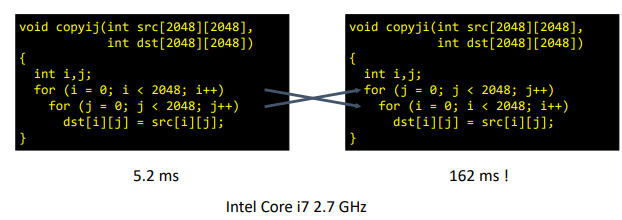
\includegraphics[width=13cm]{Pictures/e1.png}
    \caption{Access pattern time difference}
    \label{fig:example}
\end{figure}
\end{itemize}
\subsection{Performance and Asymptotic Complexity}

\begin{itemize}
    \item Constant factors matter too -often more
    \item Even exact op count does not predict performance
\end{itemize}
\subsubsection{Example: matrix-matrix multiplication}
\begin{itemize}
    \item Fundamental operation in ML, graphics, etc...: $(...)\leftarrow(...)\times(...)$\\
    \begin{figure}[htp]
        \centering
        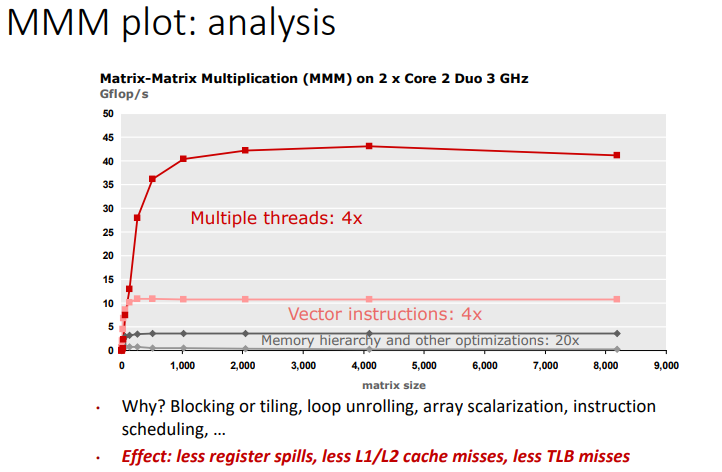
\includegraphics[width=11cm]{Pictures/e2.png}
        \caption{Matrix Multiplication: analysis}
        \label{fig:enter-label}
    \end{figure}
\end{itemize}
\subsection{Role of "Standards"}
\begin{itemize}
    \item Language standards aim to \textbf{specify unambigously} what any program
in the language does when compiled and executed. (e.g. Java)
    \item The C standards should be viewed as rather different
    \begin{itemize}
        \item Behavior frequently describes as \textbf{implementation dependent}
    \end{itemize}
    \item \textbf{Implementation defined}: unspecified behavior where each implementation documents how the choice is made
    \begin{itemize}
        \item Compiler is allowed to do \textbf{anything}, so optimizes out the code completely (newer C-compilers)
        \item Compiler implements the \textbf{most natural mapping} to the target hardware and \textbf{documents} this. (older C-compilers)
    \end{itemize}
    \textbf{A program is a set of instructions to a compiler that tell it what assembly language to generate.}
\end{itemize}

\section{Vorlesung}
\subsection{C Overview}
\begin{itemize}
    \item \textbf{No} objects, classes, traits, features, methods, or interfaces
    \item \textbf{No} expections
    \item \textbf{No} automatic memory management
    \item \textbf{Def. Pointers}: direct access to memory adresses
\end{itemize}
C is about directly building and manipulating structures in main
memory!\\ 
\subsection{Hello World in C}
\begin{figure}[htp]
    \centering
    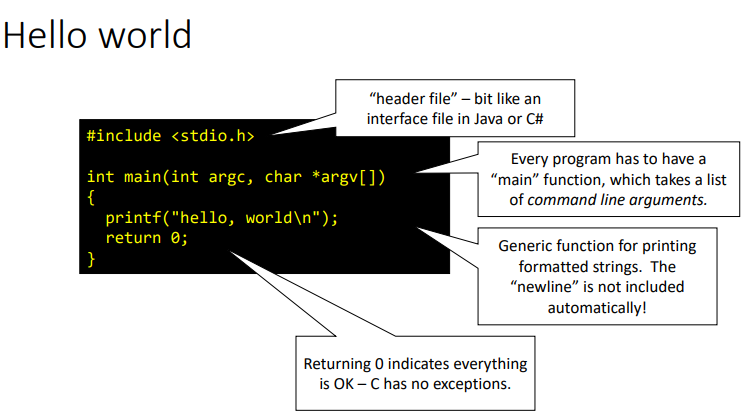
\includegraphics[width=1\linewidth]{Pictures/e3.png}
    \caption{Hello World Program in C}
\end{figure}
\subsection{Workflow in C \& GNU gcc Toolchain}
\begin{figure}[htp]
    \centering
    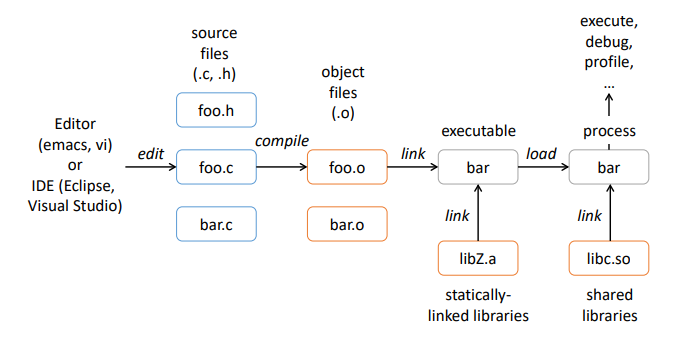
\includegraphics[width=1\linewidth]{Pictures/e4.png}
    \caption{Workflow of C}
    \label{fig:enter-label}
\end{figure}
\begin{figure}[htp]
    \centering
    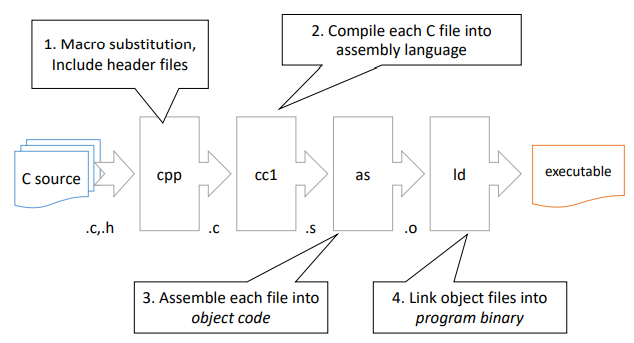
\includegraphics[width=1\linewidth]{Pictures/e5.png}
    \caption{gcc Toolchain; cpp = macro pre-processor}
    \label{fig:enter-label}
\end{figure}
\begin{tipbox}
    {Info for gcc}
    \textit{gcc exampleC.c} (produces an executable file)
    \textit{-o difName} (changes Executable name)
    \textit{-c } (compiles the program and gives the object file as output, which is used to make libraries)
    To execute executable use: \textit{./exfileName}
\end{tipbox}

\subsection{Control flow statments}
Mostly same as Java

\textit{goto Label} (controversial, but sometimes very useful)
\pagebreak

\subsection{Functions in C}
\begin{figure}[h]
    \centering
    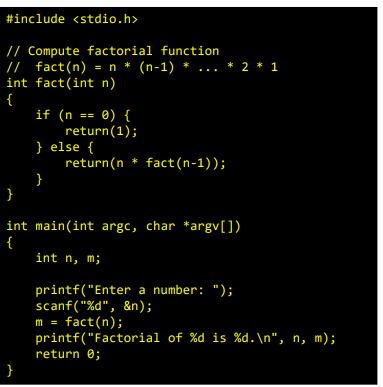
\includegraphics[width=0.75\linewidth]{Pictures/e6.png}
    \caption{Introduction functions in C}
    \label{fig:enter-label}
\end{figure}

\subsection{Basic I/O}
\subsubsection{printf()}
\begin{figure}[h]
    \centering
    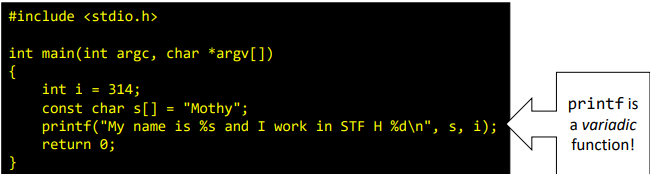
\includegraphics[width=1\linewidth]{Pictures/e7.png}
    \caption{\textit{printf}}
    \label{fig:enter-label}
\end{figure}
\%d means number in decimal
\%s for argument s
\subsection{Summary control flow}
\begin{figure}[h!]
    \centering
    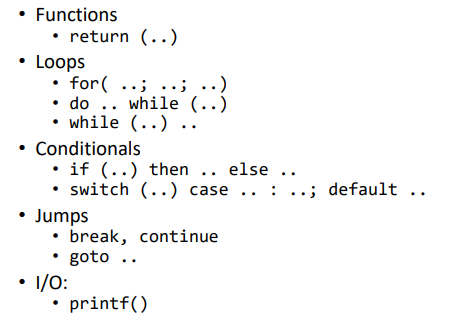
\includegraphics[width=0.7\linewidth]{Pictures/e8.png}
    \caption{Summary control flow}
    \label{fig:enter-label}
\end{figure}

\pagebreak
\subsection{Declarations in C}
\begin{figure}[!h]
    \centering
    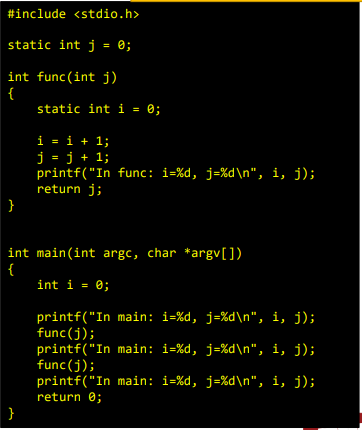
\includegraphics[width=0.75\linewidth]{Pictures/e9.png}
    \caption{Declaration example}
    \label{fig:enter-label}
\end{figure}
\begin{tipbox}
    {Info declarations}
    \begin{itemize}
        \item Declaration in block: Scope is just the block \& \textit{static} $\rightarrow$ value \textbf{persist} between calls
        \item Declaration outside block: Scope is the entire program \& \textit{static} $\rightarrow$ scope limited to the file (\textbf{compilation unit})
    \end{itemize}
\end{tipbox}
\subsubsection{Integers and floats}
\begin{figure}[htp]
    \centering
    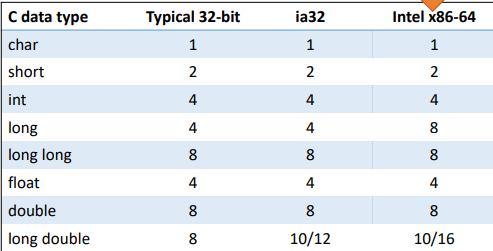
\includegraphics[width=1\linewidth]{Pictures/e10.png}
    \caption{Types and sizes}
\end{figure}
\begin{tipbox}
    {}
    Integers are \textbf{signed} by default; however use \textit{signed} \& \textit{unsigned} for clarification
\end{tipbox}
\begin{figure}[h]
        \centering
        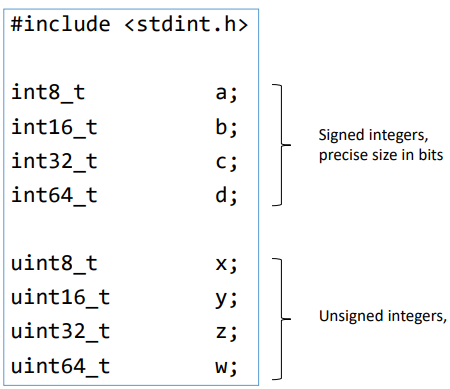
\includegraphics[width=0.7\linewidth]{Pictures/e11.png}
        \caption{C99 extended integer types}
    \end{figure}
\pagebreak
\begin{tbox}
    {Rules for conversions}
    \begin{itemize}
        \item Implicit conversions between integer types
        \item implicit conversions between floating point types
        \item Explicit conversions between anything (casts)
    \end{itemize}
\end{tbox}
\subsubsection{Booleans}
\begin{itemize}
    \item False $\rightarrow$ zero
    \item True $\rightarrow$ anything non-zero
    \item Negations ("!") turns zero into non zero and vice-versa
\end{itemize}
\pagebreak
\begin{tipbox}
    {Important}
    Any statment in C is also an expression
\end{tipbox}
\begin{figure}[h]
    \centering
    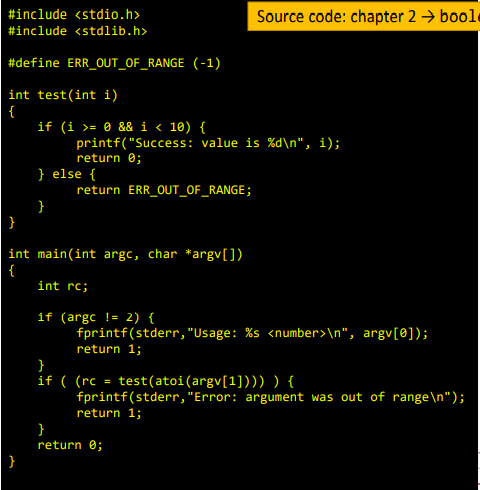
\includegraphics[width=0.7\linewidth]{Pictures/e12.png}
    \caption{Example that any statement is an expression}
    \label{fig:enter-label}
\end{figure}
\subsubsection{void}
\begin{itemize}
    \item has \textbf{no} value
    \item used for
    \begin{itemize}
        \item Untyped pointers (to raw memory):“void *"
        \item Declaring functions with no return value (procedures)
    \end{itemize}
\end{itemize}
\pagebreak
\subsection{Operators in C}
\begin{figure}[h]
    \centering
    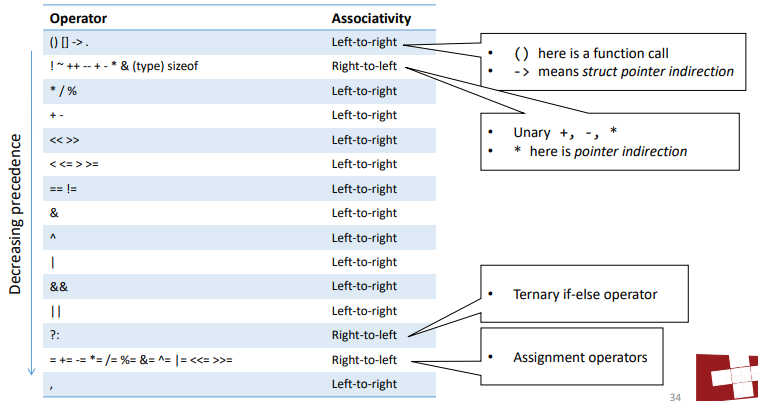
\includegraphics[width=1\linewidth]{Pictures/e13.png}
    \caption{Operators in C}
    \label{fig:enter-label}
\end{figure}
\section{Lecture (\today)}
\subsection{Arrays}
\begin{itemize}
    \item Finite vector of variables all the same type
    \item C compiler \textbf{does not} check the array bounds
    \item can be initialized when they are defined
    \begin{figure}[h!]
        \centering
        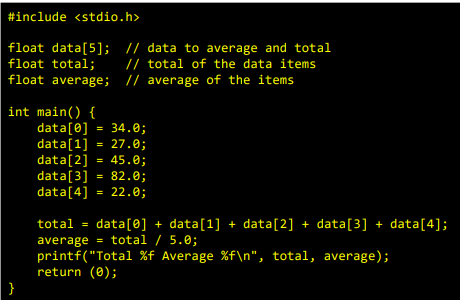
\includegraphics[width=0.75\linewidth]{Pictures/e14.png}
        \caption{Array Example}
        \label{fig:enter-label}
    \end{figure}
    \begin{figure}[h!]
        \centering
        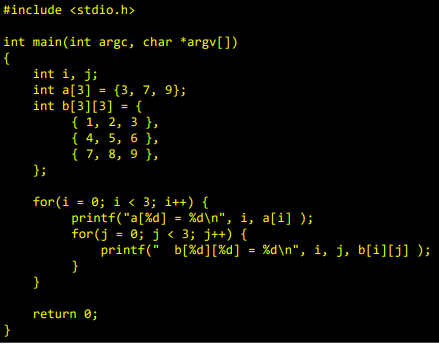
\includegraphics[width=0.75\linewidth]{Pictures/e15.png}
        \caption{Setting an array to 0 (it is \textbf{not always} initialized with 0)}
        \label{fig:enter-label}
    \end{figure}
\end{itemize}
\subsection{Strings}
\begin{itemize}
    \item C has no real string type!
    \item Array of char's terminated with null byte
    \item single quotes evaluate to byte value with ASCII numeric code
    \begin{figure}[h!]
        \centering
        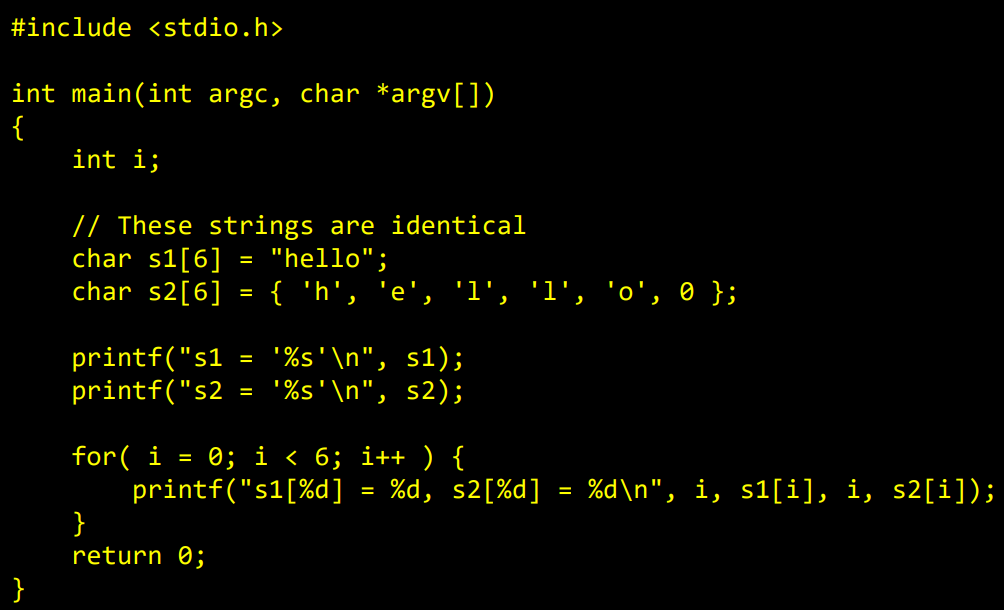
\includegraphics[width=0.75\linewidth]{Pictures/e16.png}
        \caption{"String" example C}
        \label{fig:enter-label}
    \end{figure}
\end{itemize}
\textbf{String libary functions}
\begin{itemize}
    \item usually names "strxxx()"
    \item \textbf{strcopy}(copiedValue, valueToBeCopied)
    \item \textbf{strcat}(firstPart, lastPart)
    \item \textbf{strcmp}(str1, str2)
\end{itemize}
\subsection{Bit-Shifts}
\begin{itemize}
    \item Example number: 10100010
    \item Log. Shift (unsigned numbers): $>>$ 2 := 00101000
    \item Arith. Shift (unsigned numbers): $>>$ 2 := 11101000
    \item \textbf{Undefined} behavior: shift amount $<0$ or $\ge$ word size
\end{itemize}
\subsection{Integers in C}
\subsubsection{MaxValues}
\begin{itemize}
    \item \#include $<$limits.h$>$ 
    \item Declares constants like \textit{ULONG\_MAX, LONG\_MAX, LONG\_MIN}
    \item Values platform specific
\end{itemize}
\subsubsection{Signed vs. unsigned in C}
\begin{itemize}
    \item Default: signed integers
    \item Unsigned if "U" as suffix
    \item When mixing unsigned and signed in single expression, \textbf{signed values implicitly cast to unsigned} (also for \underline{comparison} operators.
    
    \begin{figure}[h!]
        \centering
        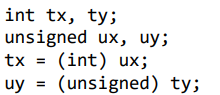
\includegraphics[width=0.5\linewidth]{Pictures/e17.png}
        \caption{Explicit casting between signed \& unsigned same as U2T and T2U}
        \label{fig:enter-label}
    \end{figure}
    \begin{figure}[h!]
        \centering
        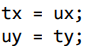
\includegraphics[width=0.2\linewidth]{Pictures/e18.png}
        \caption{Implicit casting}
        \label{fig:enter-label}
    \end{figure}    
\end{itemize}
\subsubsection{Expanding numbers (e.g. short int $\rightarrow$ int)}
\begin{itemize}
    \item \textbf{Unsigned}: zeros added
    \item \textbf{Signed}: \underline{sign extension} (copying the left most bit = sign bit)
\end{itemize}
\subsubsection{Truncating (e.g. unsigned $\rightarrow$ unsigned short)}
\begin{itemize}
    \item \textbf{Unsigned}: modulus operation
    \item \textbf{Signed}: similar to modulus
    \item For small numbers yields expected behavior
\end{itemize}
\section{Lecture (\today)}
\subsection{Addition in C}
\begin{itemize}
    \item Modular addition forms an Abelian group
    \begin{itemize}
        \item Closed under addition
        \item Commutative
        \item Associative
        \item 0 has additive identity 
        \item Every element has additive inverse
    \end{itemize}
    \item  TAdd and uAdd have \underline{identical} bit-level behavior
\end{itemize}
\subsection{Integer Multiplication in C}
\begin{itemize}
    \item Unsigned multiplication with addition forms a \textbf{commutative ring}
    \item \textbf{Signed} mutliplication
    \begin{itemize}
        \item Isomorphic algebra to unsigned multiplication and addition
        \item 
    \end{itemize}
\end{itemize}
\subsection{Division with shifts}
\textbf{Watch out}: Negative numbers divided by bit-shifting can be off by 1 (because it gets rounded towards 0 (bitwise)). 
\begin{enumerate}
    \item Case: No rounding $\implies$ Biasing (see above) has no effect
    \item Case: Rounding $\implies$ Biasing adds 1 to final result (do $(s + (1<<k)-1) >> k$ instead)
\end{enumerate}
\subsection{Summary Integer Multiplication \& Division}
\begin{itemize}
    \item Signed/unsigned multiply: $x * 2^k= x<<k$
    \item Unsigned divide: $u/2^k=u>>k$ (logic shift)
    \item Signed divide:
    \begin{itemize}
        \item $s/2^k=x>>k$ for $s>0$
        \item $s / 2k = s + (2k – 1) >> k$ (arithmetic shift) for $s < 0 $ 
    \end{itemize}
\end{itemize}
\pagebreak
\section{Lecture (\today)}
\subsection{Process address space}
\begin{itemize}
    \item OS gves each process an \underline{address space}
    \item  Contains process \underline{virtual memory}
    \begin{itemize}
        \item visible only to it
        \item each byte in memory has an address
        \item on 64 bit host: 264 bytes of virtual memory (as shown)
    \end{itemize}
    \item When the OS loads a program, it:
    \begin{itemize}
        \item \textbf{creates} an address space
        \item inspects the executable file to see what’s in it        
        \item (lazily) copies regions of the file into the right place in the address space
        \item final \underline{linking, relocation}
        \begin{figure}[H]
            \centering
            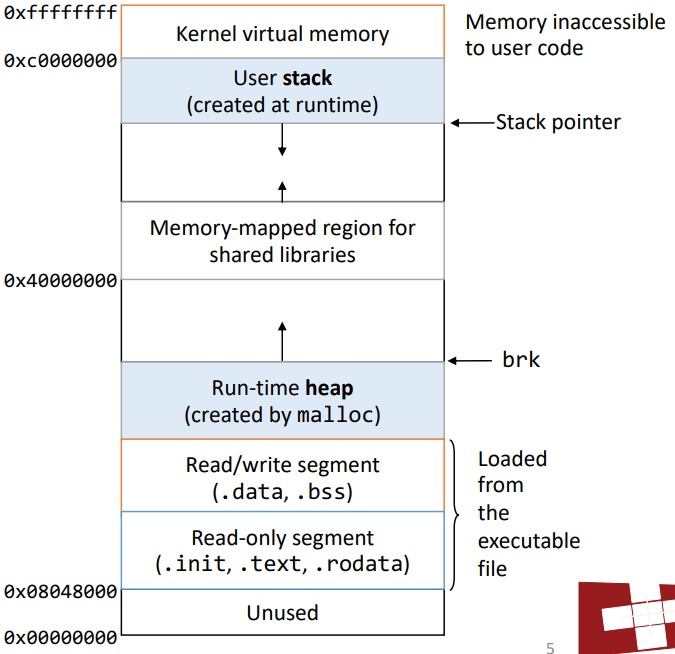
\includegraphics[width=0.65\linewidth]{Pictures/e19.png}
            \caption{Example: Loading a program}
            \label{fig:enter-label}
        \end{figure}
    \end{itemize}
    \item Stack size is \textbf{not} directly controlled by programmer
\end{itemize}
\subsection{Stack}
\begin{itemize}
    \item needed for recursions (code must be reentrant)
    \item allocated in Frames (state for single procedure (e.g. main) activation)
    \item Stack discipline (Callee returns before caller does -> main first on stack and last to go)
\end{itemize}
\begin{figure}[H]
    \centering
    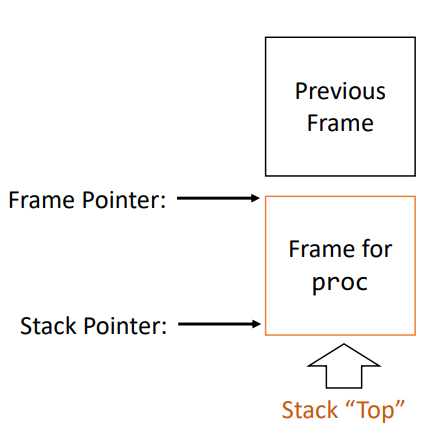
\includegraphics[width=0.5\linewidth]{Pictures/e20.png}
    \caption{Stack Frame example. contains local variables, return temp information, temp space}
    \label{fig:enter-label}
\end{figure}
\subsection{Pointer}
\textbf{Definition}: Pointer is a variable whose value is the memory address of another variable
\subsubsection{Syntax}
\begin{lstlisting}[language=C++]
type *name; // declare a pointer 
type *name = address; // declare + initialize pointer
v = *pointer // dereference pointer
*pointer = value // dereference / assign
type **doublepointer = &pointer; //initializing double pointer
v1 = **doublepointer // dereferencing double pointer
\end{lstlisting}
\subsection{Null}
\begin{itemize}
    \item A guaranteed-to-be invalid memory location
    \item \textit{typeof(NULL)} is \textit{void *}
    \item dereference \textit{NULL} $\implies$ segmentation fault
\end{itemize}
\section{Lecture (\today)}
\subsection{"simple" \textit{strcpy()}}
\begin{figure}[H]
    \centering
    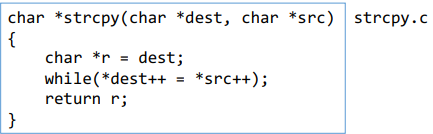
\includegraphics[width=0.75\linewidth]{Pictures/e21.png}
    \caption{Example for \textit{strcpy()} method}
    \label{fig:enter-label}
\end{figure}
\begin{itemize}
    \item Strings are arrays of characters terminated by null bytes
    \item Assigment is an expression, not a statement --- returns the value assigned
    \item Non-zero values evaluate to true, zero evaluates to false
    \item Post-increment operators bind more tightly than pointer dereference
    \item A semicolon is statement terminator, not a separator
    \item This is also a dangerous function: use strncpy() instead
\end{itemize}
\subsection{Danamically allocated memory}
\begin{itemize}
    \item Program \textbf{explicitly} requests new block of memory
    \item  Dynamically allocated memory persists until: code explicitly \textbf{deallocates} it or \textbf{garbage collector} collects it
    \item C requires \textbf{manual} memory management
\end{itemize}
\subsection{The C memory API}
\begin{itemize}
    \item \textbf{*malloc()}: Allocates a block of memory of the given size
    \begin{itemize}
        \item \textbf{assume} the memory initially contains garbage
        \item typically use \textit{sizeof()} to calculate the size you need
        \item returns a pointer to the first byte of that memory (returns 0 if it did not work $->$ check if return value = 0)
    \end{itemize}
    \begin{figure}[H]
        \centering
        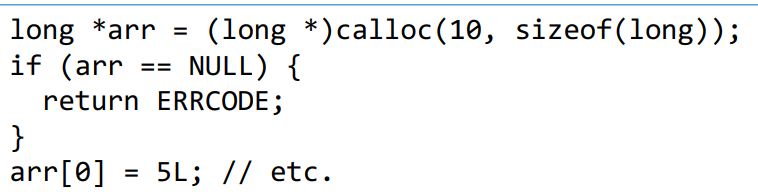
\includegraphics[width=0.6\linewidth]{Pictures/e22.png}
        \caption{Example: Use of malloc()}
        \label{fig:enter-label}
    \end{figure}
    \pagebreak
    \item \textbf{*calloc()}
    \begin{itemize}
        \item Allocates a block of memory size $(nm /times sz)$
        \item Like malloc(), a pointer to the first byte of that memory
        \item \textbf{Important}: zeroes the memory - unlike malloc()
    \end{itemize}
    \begin{figure}[H]
        \centering
        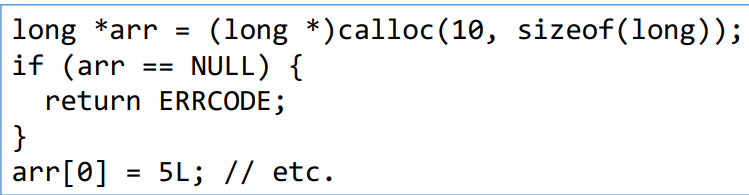
\includegraphics[width=0.75\linewidth]{Pictures/e23.png}
        \caption{Example: Use of calloc()}
        \label{fig:enter-label}
    \end{figure}

    \item \textbf{free()}
    \begin{itemize}
    \item Releases memory at the pointer
    \item Good practice to NULL the pointer after freeing (otherwise some weird things might happen when you try to use the pointer again)
\end{itemize}
\begin{figure}
    \centering
    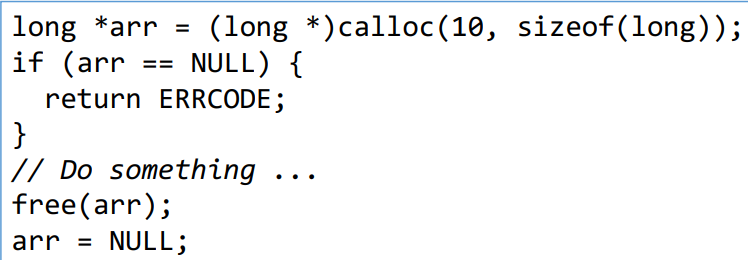
\includegraphics[width=0.75\linewidth]{Pictures/e24.png}
    \caption{Enter Caption}
    \label{fig:enter-label}
\end{figure}

\item \textbf{*realloc()}: changing the size of the block
    \begin{itemize}
        \item Allocations have \textbf{fixed} size
        \item \textbf{Always} use the new address returned
        \item Like free(), realloc() \textbf{must point} to first byte of a malloc’ed block
    \end{itemize}
    \begin{figure}[H]
        \centering
        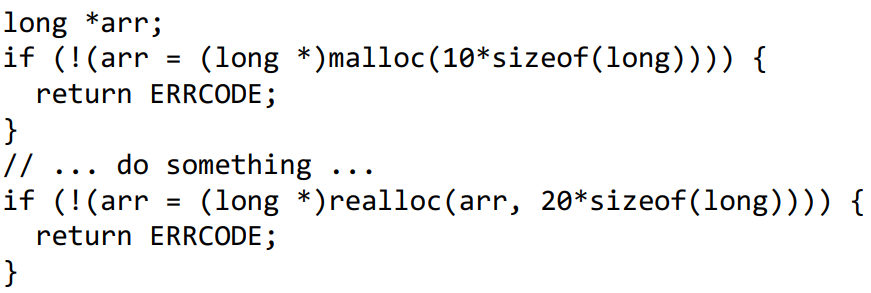
\includegraphics[width=0.75\linewidth]{Pictures/e25.png}
        \caption{Example: Use of \textit{*realloc()}}
        \label{fig:enter-label}
    \end{figure}   
\end{itemize}
\subsection{Memory Leak}
A \textbf{memory leak} happens when code fails do deallocate memory that will no longer be used (when you don't free memory).
\textbf{Implications of a leak}:
\begin{itemize}
    \item Program’s memory footprint will keep growing
    \item Especially for long-lived programs bad: might slow it down, starve other programs from memory, etc...
\end{itemize}
\subsection{Structured data}
\textbf{struct}: a C type that contains a set of fields (has no methods or constructors)


\end{document}